\documentclass[10pt]{jhwhw}
\author{Ian Malerich}
\title{Math S 373: Homework 1}
\usepackage{amssymb, amsfonts, amsmath, mathtools, graphicx, breqn, soul}
\usepackage{minted, subfig, float, scrextend, setspace, amsthm}
\usemintedstyle{friendly}

\begin{document}
\raggedright

%% Problem 1
\problem{} (10 points)
	Find the least squares polynomial of degree 2 for the data in the following
	table. Compute the error E. Graph the data and the polynomial.
	\bigbreak
	\begin{tabular}{ccccccc}
		\hline
		$x_i$ & 1.0 & 1.1 & 1.3 & 1.5 & 1.9 & 2.1 \\
		$y_i$ & 1.84 & 1.96 & 2.21 & 2.45 & 2.94 & 3.18 \\
		\hline
	\end{tabular}

\solution

	A = 
	\left[\begin{array}{ccc}
		1 & 1 & 1 \\
		1 & 1.1 & 1.1^2 \\
		1 & 1.3 & 1.3^2 \\
		1 & 1.5 & 1.5^2 \\
		1 & 1.9 & 1.9^2 \\
		1 & 2.1 & 2.1^2 \\
	\end{array} \right]
	b = 
	\left[\begin{array}{c}
		1.84 \\ 1.96 \\ 2.21 \\ 2.45 \\ 2.94 \\ 3.18 \\
	\end{array} \right]

	\bigbreak
	$A^TAa = A^Tb \Rightarrow (A^TA)^{-1}(A^TA)a = (A^TA)^{-1}A^Tb \Rightarrow
	a = (A^TA)^{-1}A^Tb$

	\begin{align*}
	a &= 
	\left[\begin{array}{ccc}
		66.841 & -90.719 & 28.748 \\
		-90.719 & 124.544 & -39.811 \\
		28.748 & -39.811 & 12.832 \\
	\end{array} \right]
	\left[\begin{array}{ccc}
		1 & 1 & 1 & 1 & 1 & 1 \\
		1 & 1.1 & 1.3 & 1.5 & 1.9 & 2.1 \\
		1 & 1.21 & 1.69 & 2.25 & 3.61 & 4.41 \\
	\end{array} \right]
	\left[\begin{array}{c}
		1.84 \\ 1.96 \\ 2.21 \\ 2.45 \\ 2.94 \\ 3.18 \\
	\end{array} \right]
	\\ &= 
	\left[\begin{array}{cccccc}
		4.86939 & 1.83451 & -2.51039 & -4.55547 & -1.74620 & 3.10816 \\
		-5.98639 & -1.89239 & 3.90693 & 6.52134 & 2.19542 & -4.74490 \\
		1.76871 & 0.48237 & -1.32035 & -2.09647 & -0.56895 & 1.773469 \\
	\end{array} \right]
	\left[\begin{array}{c}
		1.84 \\ 1.96 \\ 2.21 \\ 2.45 \\ 2.94 \\ 3.18 \\
	\end{array} \right]
	\\ &= 
	\left[\begin{array}{c}
		0.596581 \\ 1.253293 \\ -0.010853 \\
	\end{array} \right]
	\end{align*}

	This gives us the interpolating polynomial as
	$
		P_2(x) = -0.010853x^2 + 1.253293x + 0.596581
	$.

	Evaluating our initial points using our polynomial produces the results...
	\bigbreak
	\begin{tabular}{ccccccc}
		\hline
		$x_i$ & 1.0 & 1.1 & 1.3 & 1.5 & 1.9 & 2.1 \\
		$y_i$ & 1.84 & 1.96 & 2.21 & 2.45 & 2.94 & 3.18 \\
		$P(x_i)$ & 1.839 & 1.9621 & 2.2075 & 2.4521 & 2.9387 & 3.1806 \\
		$|P(x_i)-y_i|$ & -9.79e-4 & 2.0712e-3 & 2.4797e-3 & 2.1012e-3 & 1.3416e-3 & 6.3457e-4 \\
		\hline
	\end{tabular} \bigbreak
	Taking the sum of the differences finds the total error across all interpolating
	points as $E = 6.69\times 10^{-6}$.

	\bigbreak
	We can see that the least squares fit finds a polynomial which is 
	almost linear, but not quite. From both the graph below, and the error above,
	the polynomial is clearly doing a good job (though not perfect) of fitting to
	the points.
	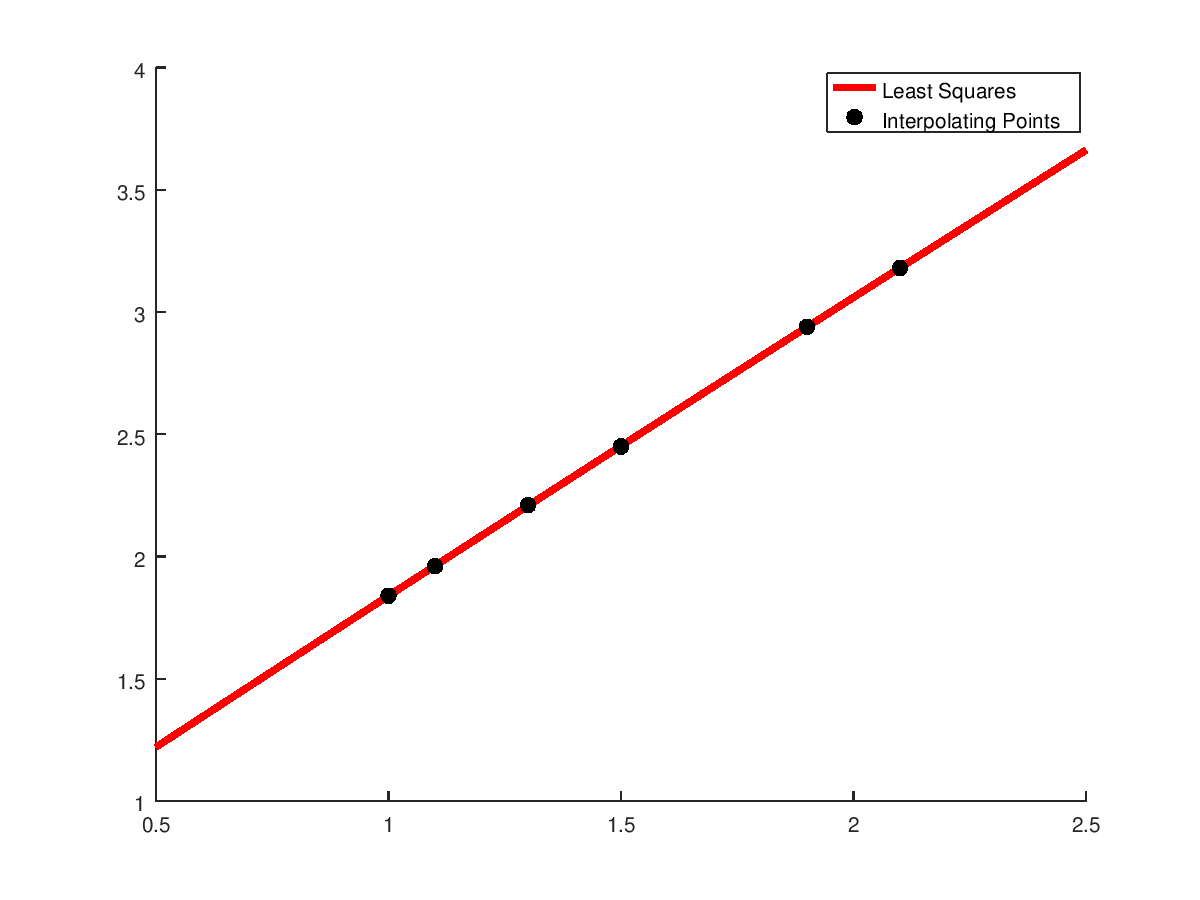
\includegraphics[scale=0.75]{p1}

%% Problem 2
\problem{} (20 points)

	\begin{enumerate}
		\item Find the least squares polynomial of degree 2 for the following function
			$f(x)$ on the indicated interval
			$$
				f(x) = e^x,\ [-1,1]
			$$
			Compute the error E. Graph the function and the polynomial.
		\item Repeat (a) with Legendre Polynomials.
	\end{enumerate}

\solution

	\part
	\begin{tabular}{cccc}
		\hline
		$x_i$ & -1 & 0 & 1 \\
		$y_i$ & \frac{1}{e} & 1 & e
		\hline
	\end{tabular}

	\bigbreak
	$
	A = 
	\left[\begin{array}{ccc}
		1 & 1 & 1 \\
		1 & 1.1 & 1.1^2 \\
		1 & 1.3 & 1.3^2 \\
		1 & 1.5 & 1.5^2 \\
		1 & 1.9 & 1.9^2 \\
		1 & 2.1 & 2.1^2 \\
	\end{array} \right]
	b = 
	\left[\begin{array}{c}
		1.84 \\ 1.96 \\ 2.21 \\ 2.45 \\ 2.94 \\ 3.18 \\
	\end{array} \right]
	$

	\part

%% Problem 3
\problem{} (20 points)

	\begin{enumerate}
		\item Use the zeros of $\overline{T}_4$ to construct an interpolating polynomial of degree
			3 for the following function on the interval $[-1,1]$:
			$$
				f(x) = e^x
			$$
			Find a bound for the maximum error of the approximation.
		\item Repeat (a) on interval $[0, 2]$.
	\end{enumerate}

\solution

	TODO

%% Problem 4
\problem{} (20 points)
	Find all the Chebyshev rational approximations of degree 2 for $f(x) = e^{-x}$.
	Graph the function and the polynomial. (Use MATLAB routines on classpage)

\solution

	TODO

%% Problem 5
\problem{} (30 points) (Use MATLAB routines on classpage)

	\begin{enumerate}
		\item Find the continous least squares trigonometric polynomial $S_3(x)$ for
			$f(x) = e^x$ on $[-\pi,\pi]$.
		\item Find the discrete least squares trigonometric polynomials $S_n(x)$ for
			$f(x) = e^x$ on $[-\pi, \pi]$ with $n=3, m=6$.
		\item Find the trigonometric interpolating polynomial $S_n(x)$ for 
			$f(x) = e^x$ on $[-\pi, \pi]$ with $n=8$.
	\end{enumerate}

\solution

	TODO

\end{document}
